%%%%%%%%%%%%%%%%%%%%%%%%%%%%%%%%%%%%%%%%%
% Beamer Presentation
% LaTeX Template
% Version 1.0 (10/11/12)
%
% This template has been downloaded from:
% http://www.LaTeXTemplates.com
%
% License:
% CC BY-NC-SA 3.0 (http://creativecommons.org/licenses/by-nc-sa/3.0/)
%
%%%%%%%%%%%%%%%%%%%%%%%%%%%%%%%%%%%%%%%%%

%----------------------------------------------------------------------------------------
%	PACKAGES AND THEMES
%----------------------------------------------------------------------------------------

\documentclass[UTF8,aspectratio=169,14pt]{ctexbeamer}

\usepackage{hyperref}
\hypersetup{
	colorlinks=true,
	linkcolor=red,
	anchorcolor=blue,
	citecolor=green
}

\mode<presentation> {
	
	% The Beamer class comes with a number of default slide themes
	% which change the colors and layouts of slides. Below this is a list
	% of all the themes, uncomment each in turn to see what they look like.
	
	%\usetheme{default}
	%\usetheme{AnnArbor}
	%\usetheme{Antibes}
	%\usetheme{Bergen}
	%\usetheme{Berkeley}
	%\usetheme{Berlin}
	%\usetheme{Boadilla}
	%\usetheme{CambridgeUS}
	%\usetheme{Copenhagen}
	%\usetheme{Darmstadt}
	%\usetheme{Dresden}
	%\usetheme{Frankfurt}
	%\usetheme{Goettingen}
	%\usetheme{Hannover}
	%\usetheme{Ilmenau}
	%\usetheme{JuanLesPins}
	%\usetheme{Luebeck}
	\usetheme{Madrid}
	%\usetheme{Malmoe}
	%\usetheme{Marburg}
	%\usetheme{Montpellier}
	%\usetheme{PaloAlto}
	%\usetheme{Pittsburgh}
	%\usetheme{Rochester}
	%\usetheme{Singapore}
	%\usetheme{Szeged}
	%\usetheme{Warsaw}
	
	% As well as themes, the Beamer class has a number of color themes
	% for any slide theme. Uncomment each of these in turn to see how it
	% changes the colors of your current slide theme.
	
	%\usecolortheme{albatross}
	%\usecolortheme{beaver}
	%\usecolortheme{beetle}
	%\usecolortheme{crane}
	%\usecolortheme{dolphin}
	%\usecolortheme{dove}
	%\usecolortheme{fly}
	%\usecolortheme{lily}
	%\usecolortheme{orchid}
	%\usecolortheme{rose}
	%\usecolortheme{seagull}
	%\usecolortheme{seahorse}
	%\usecolortheme{whale}
	%\usecolortheme{wolverine}
	
	%\setbeamertemplate{footline} % To remove the footer line in all slides uncomment this line
	%\setbeamertemplate{footline}[page number] % To replace the footer line in all slides with a simple slide count uncomment this line
	
	%\setbeamertemplate{navigation symbols}{} % To remove the navigation symbols from the bottom of all slides uncomment this line
}

\usepackage{graphicx} % Allows including images
\graphicspath{{./figs/}}
\usepackage{booktabs} % Allows the use of \toprule, \midrule and \bottomrule in tables
\usepackage{longtable}
\usepackage{listings}
\usepackage{xcolor}
\lstset{numbers=left, %设置行号位置
	numberstyle=\tiny, %设置行号大小
	keywordstyle=\color{blue}, %设置关键字颜色
	commentstyle=\color[cmyk]{1,0,1,0}, %设置注释颜色
	frame=single, %设置边框格式
	escapeinside=``, %逃逸字符(1左面的键),用于显示中文
	%breaklines, %自动折行
	extendedchars=false, %解决代码跨页时,章节标题,页眉等汉字不显示的问题
	xleftmargin=2em,xrightmargin=2em, aboveskip=1em, %设置边距
	tabsize=4, %设置tab空格数
	showspaces=false %不显示空格
}
% Fonts
% \usepackage{libertine}
% \setmonofont{Courier}
\setCJKsansfont[ItalicFont=Noto Serif CJK SC Black, BoldFont=Noto Sans CJK SC Black]{Noto Sans CJK SC}

%\def\imagepath{./resources/graphics}
%\usepackage[imagepath=\imagepath]{ditaa}
%\graphicspath{ {\imagepath/} }


%\usepackage{pgfpages}
%\setbeameroption{show notes on second screen}
%%----------------------------------------------------------------------------------------
%	TITLE PAGE
%----------------------------------------------------------------------------------------

\title[第10讲]{第十讲:进程和线程控制} % The short title appears at the bottom of every slide, the full title is only on the title page
\subtitle{第10.1.5节:rCore进程和线程控制}
\author{向勇、陈渝、李国良} % Your name
\institute[清华大学] % Your institution as it will appear on the bottom of every slide, may be shorthand to save space
{
	清华大学计算机系 \\ % Your institution for the title page
	\medskip
	\textit{xyong,yuchen,liguoliang@tsinghua.edu.cn} % Your email address
}
\date{\today} % Date, can be changed to a custom date


\begin{document}
%----------------------------------------------
\begin{frame}
\titlepage % Print the title page as the first slide
\end{frame}
%----------------------------------------------
\begin{frame}
\frametitle{提纲} % Table of contents slide, comment this block out to remove it
\tableofcontents % Throughout your presentation, if you choose to use \section{} and \subsection{} commands, these will automatically be printed on this slide as an overview of your presentation
\end{frame}
%----------------------------------------------
%%	PRESENTATION SLIDES
%----------------------------------------------
%------------------------------------------------
\section{第10.1.5节:rCore进程和线程控制}% Sections can be created in order to organize your presentation into discrete blocks, all sections and subsections are automatically printed in the table of contents as an overview of the talk
%------------------------------------------------
\subsection{进程和线程控制块} % A subsection can be created just before a set of slides with a common theme to further break down your presentation into chunks
%------------------------------------------------
\begin{frame}[fragile]
    \frametitle{rCore进程控制块结构}
    \framesubtitle{rCore/kernel/src/process/structs.rs}
%% figure
    \begin{figure}
    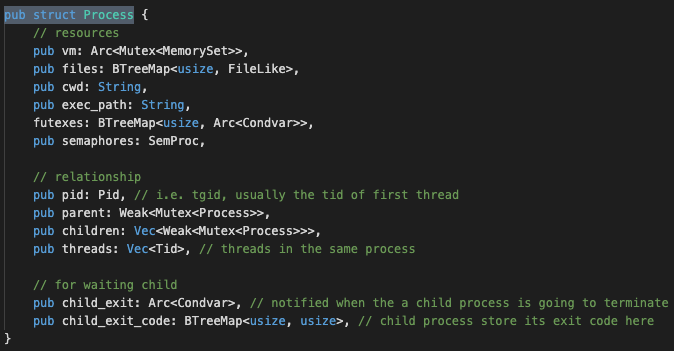
\includegraphics[width=0.8\linewidth]{figs/process.png}
%   \caption{xxxx}
    \end{figure}
\end{frame}
% #### 进程和线程数据结构
% 
% ##### 1-rCore的进程控制块结构struct Process
% 
% https://github.com/rcore-os/rCore/blob/master/kernel/src/process/structs.rs#L61
% /Users/xyong/github/rCore/kernel/src/process/structs.rs
% Line 61
% pub struct Process
% 
% ![process](figs/process.png)
% 
% /Users/xyong/github/rCore/kernel/src/process/structs.rs
% Line 42:
% pub struct Pid(usize);
% 
%------------------------------------------------
\begin{frame}[fragile]
    \frametitle{rCore内存地址空间结构}
%\end{frame}
%------------------------------------------------
% ##### 2-rCore的内存地址空间结构MemorySet
 	\begin{block}{rCore/kernel/src/memory.rs}
%% figure
    \begin{figure}
    
\includegraphics[width=1.0\linewidth]{figs/type-MemorySet.png}
%   \caption{xxxx}
    \end{figure}
 	\end{block}

% /Users/xyong/github/rCore/kernel/src/memory.rs
% Line 29:
% ```rust
% pub type MemorySet = rcore_memory::memory_set::MemorySet<PageTableImpl>;
% ```

 	\begin{block}{rCore/kernel/src/arch/riscv/paging.rs}
%    \subframetitle{rCore/kernel/src/arch/riscv/paging.rs}
%% figure
    \begin{figure}
    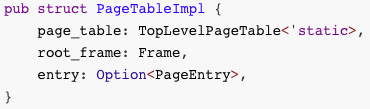
\includegraphics[width=0.65\linewidth]{figs/PageTableImpl.png}
%   \caption{xxxx}
    \end{figure}
 	\end{block}

% /Users/xyong/github/rCore/kernel/src/arch/riscv/paging.rs
% Line 20:
% pub struct PageTableImpl
% ```rust
% pub struct PageTableImpl {
%     page_table: TopLevelPageTable<'static>,
%     root_frame: Frame,
%     entry: Option<PageEntry>,
% }
% ```
\end{frame}
%------------------------------------------------
\begin{frame}[fragile]
    \frametitle{rCore内存地址空间结构}
%\end{frame}
%------------------------------------------------
 	\begin{block}{rCore/crate/memory/src/memory\_set/mod.rs}
%    \subframetitle{rCore/crate/memory/src/memory\_set/mod.rs}
%% figure
    \begin{figure}
    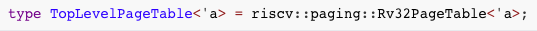
\includegraphics[width=1.0\linewidth]{figs/TopLevelPageTable.png}
%   \caption{xxxx}
    \end{figure}
 	\end{block}

% Line 16:
% ```rust
% type TopLevelPageTable<'a> = riscv::paging::Rv32PageTable<'a>;
% ```

 	\begin{block}{riscv/src/paging/multi\_level.rs}
%    \subframetitle{riscv/src/paging/multi\_level.rs}
%% figure
    \begin{figure}
    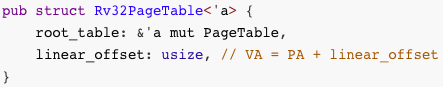
\includegraphics[width=0.7\linewidth]{figs/Rv32PageTable.png}
%   \caption{xxxx}
    \end{figure}
 	\end{block}

% /Users/xyong/github/riscv/src/paging/multi_level.rs
% Line 8:
% pub struct Rv32PageTable
% ```rust
% pub struct Rv32PageTable<'a> {
%     root_table: &'a mut PageTable,
%     linear_offset: usize, // VA = PA + linear_offset
% }
% ```

\end{frame}
%------------------------------------------------
\begin{frame}[fragile]
    \frametitle{rCore内存地址空间结构}
%\end{frame}
%------------------------------------------------

 	\begin{block}{rCore/crate/memory/src/paging/mod.rs}
% 	\framesubtitle{rCore/crate/memory/src/paging/mod.rs}
%% figure
    \begin{figure}
    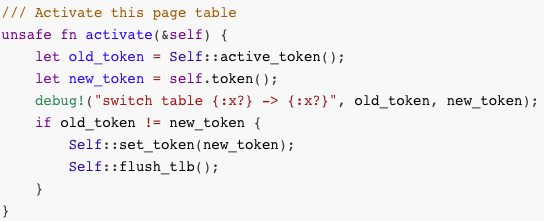
\includegraphics[width=0.7\linewidth]{figs/fn-activate.png}
%   \caption{xxxx}
    \end{figure}
 	\end{block}

% /Users/xyong/github/rCore/crate/memory/src/paging/mod.rs
% Line 111:
% unsafe fn activate(&self)
% 
% ```rust
%     /// Activate this page table
%     unsafe fn activate(&self) {
%         let old_token = Self::active_token();
%         let new_token = self.token();
%         debug!("switch table {:x?} -> {:x?}", old_token, new_token);
%         if old_token != new_token {
%             Self::set_token(new_token);
%             Self::flush_tlb();
%         }
%     }
% ```
 	\begin{block}{rCore/kernel/src/arch/riscv/paging.rs}
%    \subframetitle{rCore/kernel/src/arch/riscv/paging.rs}
%% figure
    \begin{figure}
    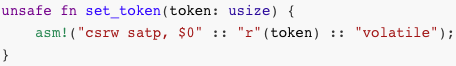
\includegraphics[width=0.6\linewidth]{figs/fn-set_token.png}
%   \caption{xxxx}
    \end{figure}
 	\end{block}

% /Users/xyong/github/rCore/kernel/src/arch/riscv/paging.rs
% Line 258:
% unsafe fn set_token(token: usize)
% ```rust
%     unsafe fn set_token(token: usize) {
%         asm!("csrw satp, $0" :: "r"(token) :: "volatile");
%     }
% ```
% 
\end{frame}
%------------------------------------------------
\begin{frame}[fragile]
    \frametitle{rCore线程控制块}
    \framesubtitle{rCore/kernel/src/process/structs.rs}
%% figure
    \begin{figure}
    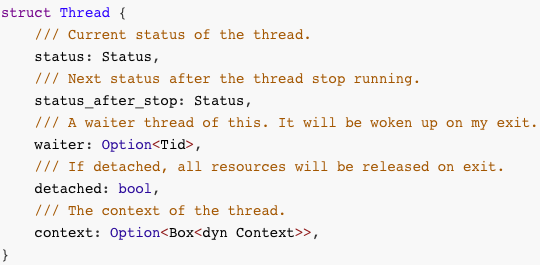
\includegraphics[width=0.9\linewidth]{figs/struct-Thread.png}
%   \caption{xxxx}
    \end{figure}

\end{frame}
%------------------------------------------------
% ##### 3-线程
% /Users/xyong/github/rCore/kernel/src/process/structs.rs
% Line 28
% pub struct Thread
% 
% https://github.com/rcore-os/rcore-thread/blob/master/src/thread_pool.rs#L8
% struct Thread
% /Users/xyong/github/rcore-thread/src/thread_pool.rs
% ```rust
% struct Thread {
%     /// Current status of the thread.
%     status: Status,
%     /// Next status after the thread stop running.
%     status_after_stop: Status,
%     /// A waiter thread of this. It will be woken up on my exit.
%     waiter: Option<Tid>,
%     /// If detached, all resources will be released on exit.
%     detached: bool,
%     /// The context of the thread.
%     context: Option<Box<dyn Context>>,
% }
% ```
% 
% https://github.com/rcore-os/rcore-thread/blob/master/src/thread_pool.rs#L25
% pub enum Status
% 
% https://doc.rust-lang.org/src/std/thread/mod.rs.html#1052
% Line 1054:
% fn new() -> ThreadId
% 
% /Users/xyong/github/rCore/kernel/src/process/mod.rs
% Line 106:
% pub fn thread_manager() -> &'static ThreadPool
% 
%------------------------------------------------
\subsection{线程状态转换} % A subsection can be created just before a set of slides with a common theme to further break down your presentation into chunks
%------------------------------------------------
\begin{frame}[fragile]
    \frametitle{线程状态数据结构}
    \framesubtitle{rcore-thread/src/thread\_pool.rs}
%% figure
    \begin{figure}
    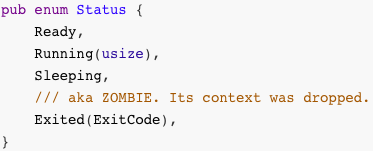
\includegraphics[width=0.7\linewidth]{figs/enum-Status.png}
%   \caption{xxxx}
    \end{figure}

\end{frame}
%------------------------------------------------
% #### 线程状态转换
% 
% ##### 4-线程状态数据结构
% 
% /Users/xyong/github/rcore-thread/src/thread_pool.rs
% 
% ```rust
% pub enum Status {
%     Ready,
%     Running(usize),
%     Sleeping,
%     /// aka ZOMBIE. Its context was dropped.
%     Exited(ExitCode),
% }
% ```
%------------------------------------------------

\begin{frame}[fragile]
    \frametitle{线程状态转换}
    \framesubtitle{rcore-thread/src/thread\_pool.rs}
%% figure
    \begin{figure}
    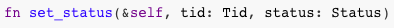
\includegraphics[width=0.6\linewidth]{figs/fn-set-status.png}
%   \caption{xxxx}
    \end{figure}

%% figure
    \begin{figure}
    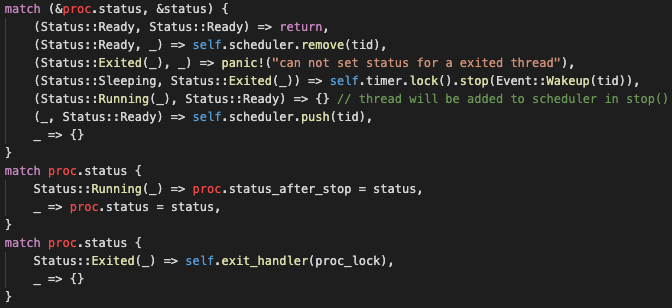
\includegraphics[width=0.8\linewidth]{figs/set-status.png}
%   \caption{xxxx}
    \end{figure}

\end{frame}
%------------------------------------------------
% ##### 4-线程状态转换
% 
% /Users/xyong/github/rcore-thread/src/thread_pool.rs
% 
% ```rust
% fn set_status(&self, tid: Tid, status: Status)
% ```
% 
% ![set-status](figs/set-status.png)
% 
%------------------------------------------------
\subsection{线程上下文切换} % A subsection can be created just before a set of slides with a common theme to further break down your presentation into chunks
%------------------------------------------------
\begin{frame}[fragile]
    \frametitle{线程上下文切换数据结构}
%    \subframetitle{TrapFrame}
%% figure
    \begin{figure}
    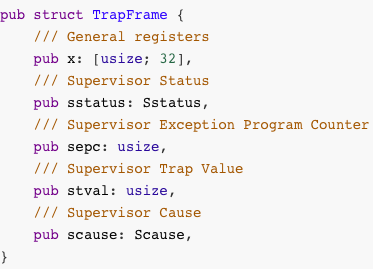
\includegraphics[width=0.6\linewidth]{figs/struct-TrapFrame.png}
%   \caption{xxxx}
    \end{figure}

在陷入异常时向栈中压入的内容,由 trap.S 的 \_\_alltraps 构建。

\end{frame}

% #### 线程上下文切换
% 
% ##### 5-上下文切换数据结构
% 
% /Users/xyong/github/rCore/docs/2_OSLab/g2/context.md
% 上下文切换的文档
% 
% 相关数据结构
% 
% 
% 1. `TrapFrame`:
% 
%     ```rust
%     pub struct TrapFrame {
%         /// General registers
%         pub x: [usize; 32],
%         /// Supervisor Status
%         pub sstatus: Sstatus,
%         /// Supervisor Exception Program Counter
%         pub sepc: usize,
%         /// Supervisor Trap Value
%         pub stval: usize,
%         /// Supervisor Cause
%         pub scause: Scause,
%     }
%     ```
% 
%     在陷入异常时向栈中压入的内容,由 [trap.S](../../../kernel/src/arch/aarch64/interrupt/trap.S#L92) 的 `__alltraps` 构建。
% 

%------------------------------------------------
\begin{frame}[fragile]
    \frametitle{线程上下文切换数据结构}
%    \subframetitle{ContextData}
%% figure
    \begin{figure}
    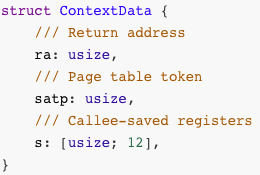
\includegraphics[width=0.55\linewidth]{figs/struct-ContextData.png}
%   \caption{xxxx}
    \end{figure}

执行上下文切换时向栈中压入的内容,由 $\_\_switch()$ 函数构建。

\end{frame}

% 2. `ContextData`:
% 
%     ```rust
%     struct ContextData {
%         /// Return address
%         ra: usize,
%         /// Page table token
%         satp: usize,
%         /// Callee-saved registers
%         s: [usize; 12],
%     }
%     ```
% 
%     执行上下文切换时向栈中压入的内容,由 `__switch()` 函数构建。
% 

%------------------------------------------------
\begin{frame}[fragile]
    \frametitle{线程上下文切换数据结构}
%    \framesubtitle{InitStack}
%% figure
    \begin{figure}
    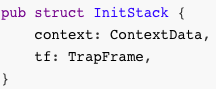
\includegraphics[width=0.5\linewidth]{figs/struct-InitStack.png}
%   \caption{xxxx}
    \end{figure}

对于新创建的线程,不仅要向栈中压入 ContextData 结构,还需手动构造 TrapFrame 结构。为了方便管理就定义了 InitStack 包含这两个结构体。

\end{frame}

% 3. `InitStack`:
% 
%     ```rust
%     pub struct InitStack {
%         context: ContextData,
%         tf: TrapFrame,
%     }
%     ```
% 
%     对于新创建的线程,不仅要向栈中压入 `ContextData` 结构,还需手动构造 `TrapFrame` 结构。为了方便管理就定义了 `InitStack` 包含这两个结构体。
% 

%------------------------------------------------
\begin{frame}[fragile]
    \frametitle{线程上下文切换数据结构}
%    \framesubtitle{Context}
%% figure
    \begin{figure}
    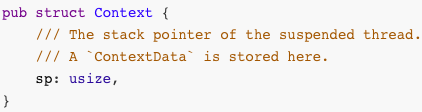
\includegraphics[width=0.9\linewidth]{figs/struct-Context.png}
%   \caption{xxxx}
    \end{figure}

每个进程控制块 Process 都会维护一个平台相关的 Context 对象。

\end{frame}

% 4. `Context`:
% 
%     ```rust
%     pub struct Context {
%         /// The stack pointer of the suspended thread.
%         /// A `ContextData` is stored here.
%         sp: usize,
%     }
%   ```
% 
%     每个进程控制块 `Process` ([kernel/src/process/context.rs](../../../kernel/src/process/structs.rs#L13)) 都会维护一个平台相关的 `Context` 对象。
% 
%------------------------------------------------
\begin{frame}[fragile]
    \frametitle{切换函数}
    \framesubtitle{rCore/kernel/src/process/structs.rs}
%% figure
    \begin{figure}
    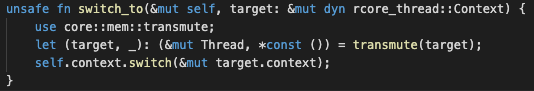
\includegraphics[width=1.0\linewidth]{figs/switch-to.png}
%   \caption{xxxx}
    \end{figure}
\end{frame}

\begin{frame}[fragile]
    \frametitle{切换函数}
    \framesubtitle{rCore/kernel/src/arch/riscv/context.rs}
%% figure
    \begin{figure}
    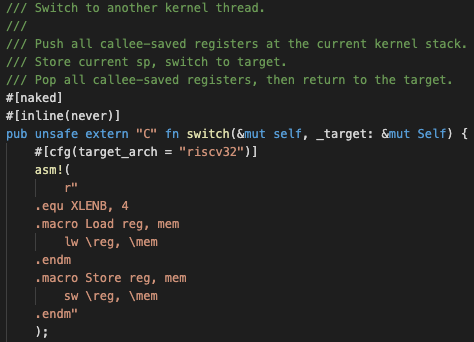
\includegraphics[width=0.6\linewidth]{riscv-32-switch.png}
%   \caption{xxxx}
    \end{figure}

\end{frame}
%------------------------------------------------
% ##### 6-切换函数
% 
% /Users/xyong/github/rCore/kernel/src/process/structs.rs
% Line 89:
% 
% ![switch-to](figs/switch-to.png)
% 
% /Users/xyong/github/rCore/kernel/src/arch/riscv/context.rs
% Line 141:
% 
% ![riscv-32-switch](figs/riscv-32-switch.png)
% 
%------------------------------------------------
\begin{frame}[fragile]
    \frametitle{线程切换过程}
    \framesubtitle{rcore-thread/src/processor.rs}
%% figure
    \begin{figure}
    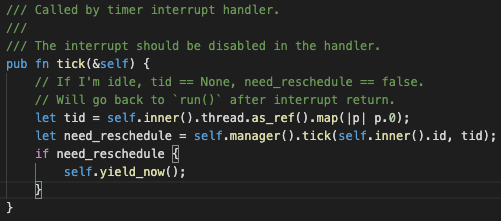
\includegraphics[width=1.0\linewidth]{figs/fn-tick.png}
%   \caption{xxxx}
    \end{figure}
\end{frame}

\begin{frame}[fragile]
    \frametitle{线程切换过程}
    \framesubtitle{rcore-thread/src/scheduler/mod.rs}
%% figure
    \begin{figure}
    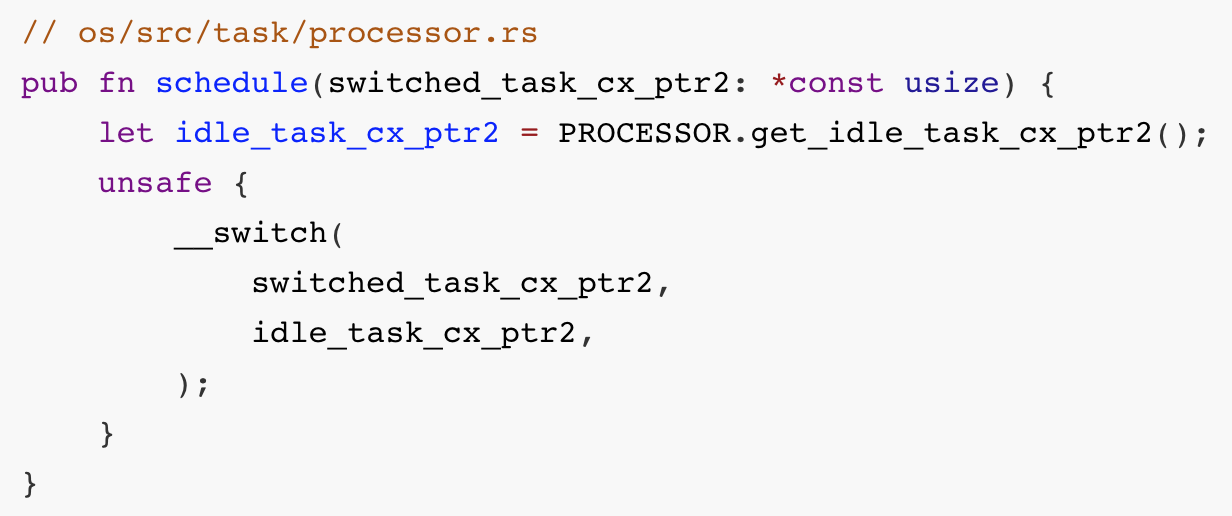
\includegraphics[width=0.65\linewidth]{figs/scheduler.png}
%   \caption{xxxx}
    \end{figure}

\end{frame}
%------------------------------------------------
% ##### 7-线程切换过程
% 
% /Users/xyong/github/rcore-thread/src/processor.rs
% 
% ![fn-tick](figs/fn-tick.png)
% 
% /Users/xyong/github/rcore-thread/src/scheduler/mod.rs
% 
% ![scheduler](figs/scheduler.png)
% 
%------------------------------------------------
\subsection{进程和线程控制接口} % A subsection can be created just before a set of slides with a common theme to further break down your presentation into chunks
%------------------------------------------------
\begin{frame}[fragile]
    \frametitle{进程管理的系统调用}
    \framesubtitle{rCore/kernel/src/syscall/proc.rs}
%% figure
    \begin{figure}
    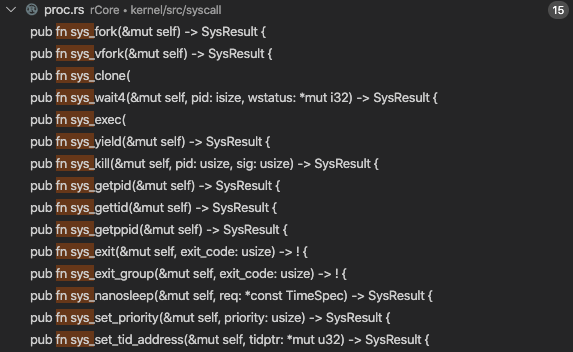
\includegraphics[width=0.7\linewidth]{figs/proc-syscall.png}
%   \caption{xxxx}
    \end{figure}

\end{frame}
% #### 进程和线程控制接口
% 
% ##### 8-进程控制系统调用
% 
% /Users/xyong/github/rCore/kernel/src/syscall/proc.rs
% 与进程管理相关的系统调用
% 
% /Users/xyong/github/rCore/kernel/src/syscall/proc.rs
% fn sys_
% 
% ![proc-syscall](figs/proc-syscall.png)
% 
%------------------------------------------------
\begin{frame}[fragile]
    \frametitle{内核中线程模块接口}
    \framesubtitle{rcore-thread/src/std\_thread.rs}
%% figure
    \begin{figure}
    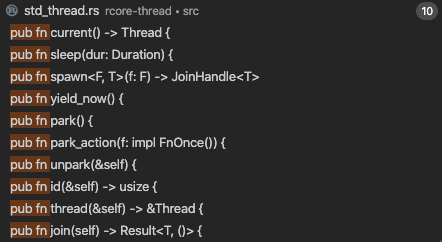
\includegraphics[width=0.7\linewidth]{figs/rcore-thread.png}
%   \caption{xxxx}
    \end{figure}

\end{frame}
%------------------------------------------------
% ##### 9-线程模块接口
% /Users/xyong/github/rcore-thread/src/std_thread.rs
% 
% ![rcore-thread](figs/rcore-thread.png)
% 
% https://doc.rust-lang.org/std/thread/#functions
% 
% ![thread-function](figs/thread-function.png)
% 
% 
%----------------------------------------------
\end{document}
